\documentclass[journal=jpcbfk,manuscript=article,layout=twocolumn]{achemso}

\usepackage[version=3]{mhchem}
\usepackage[T1]{fontenc}
\newcommand*\mycommand[1]{\texttt{\emph{#1}}}
\newcommand{\todo}[1]{\textcolor{red}{#1}}

\usepackage{rotating}
\usepackage{upgreek}                            
\usepackage{xcolor}
\usepackage{booktabs}
\usepackage{multirow}
\usepackage{lmodern}
\usepackage{microtype}
\usepackage{xr}
\usepackage{soul} % for highlights with \hl{} 

\usepackage[]{hyperref}

\author{Batuhan Kav}
\email{b.kav@fz-juelich.de}
\affiliation[Forschungszentrum J\"ulich]{Institute of Complex Systems: Structural Biochemistry, Forschungszentrum J\"ulich, 52425 J\"ulich, Germany}

%\author{Markus S. Miettinen}
%\affiliation[Max Planck Institute of Colloids and Interfaces]{Department of Theory and Bio-Systems, Max Planck Institute of Colloids and Interfaces, 14424 Potsdam, Germany}

%\author{O. H. Samuli Ollila}
%\email{samuli.ollila@helsinki.fi}
%\homepage[]{Your web page}
%\affiliation[University of Helsinki]{Institute of Biotechnology, University of Helsinki, Finland}
%\alsoaffiliation[Czech Academy of Sciences]{Institute of Organic Chemistry and Biochemistry of the  Czech Academy of Sciences, Flemingovo n\'{a}m. 542/2, CZ-16610 Prague 6, Czech Republic}

\title{NMRlipids IV: Polarizable Lipid Force Fields}

\begin{document}

\begin{abstract}
This work is part of the NMRlipids open collaboration (\url{nmrlipids.blogspot.fi}).
\end{abstract}

\maketitle

\section{Introduction}
%\date{\today}
So far, the NMRlipids community has focused on the performance of non-polarizable lipid force fields. As the inclusion of polarizability, both implicitly and explicitly, is getting more popular, I think a systematic review and benchmark study of the polarizable force fields would be useful for the entire lipid simulation community.

In a recent \href{http://nmrlipids.blogspot.fi/2018/04/new-nmrlipids-related-publication.html}{NMRlipids-based} publication~\cite{Melcr:2018a} electronic polarizability was included \emph{implicitly}. The results showed a great improvement on the calculated C--H bond order parameters' response to added CaCl$_{2}$. This suggests that including polarizability, even implicitly, can significantly improve performance.

In the present project, the idea is to focus on \emph{explicit} polarization.
At the moment, there are three main polarizable lipid force fields with explicit electronic polarization: CHARMM-Drude~\cite{li2017drude}, AMOEBA~\cite{chu2018anionicpolarizable,chu2018polarizable}, and CHARMM-Fluctuating Charge (FQ)~\cite{lucas2012charge}. It is possible to obtain force field parameters and run them on GROMACS, AMBER, and CHARMM, respectively. Therefore, we need to have access to GROMACS, CHARMM, and AMBER MD engines unless someone ports all of these force fields to GROMACS.

In the following, I aim to give a glimpse of what is available and how
is the performance of the aforementioned polarizable models.
Please note that in all figures presented below, the full captions from the original publications are reproduced for convenience.

%\section{Available Literature}

In the CHARMM-Drude force field, which is based on the classical Drude oscillator, a
maximum-entropy method has been employed to match the experimental NMR order
parameters. As of today, cholesterol, DPPC, DMPC, DLPC, POPC, DOPC, DPPE, POPE, and DOPE
lipids have been parametrized. Furthermore, within the same force field there
are force field parameters for ions which we can further test. Fig.~\ref{fig:drudedppc} shows the NMR deuterium order parameters for the DPPC bilayer simulated by Li~\textit{et al.}~\cite{li2017drude}.
Note that they do not report the signs of the order parameters.
Second observation is that in the Drude force
field the order parameters have, in most carbons, larger absolute values than in the original
CHARMM36 force field.

Figures~\ref{fig:drudepopc} and~\ref{fig:drudepope} show
the order parameters for POPC and POPE bilayers
in the Drude polarizable force field.

\begin{figure}[!hbt]
  \centering
  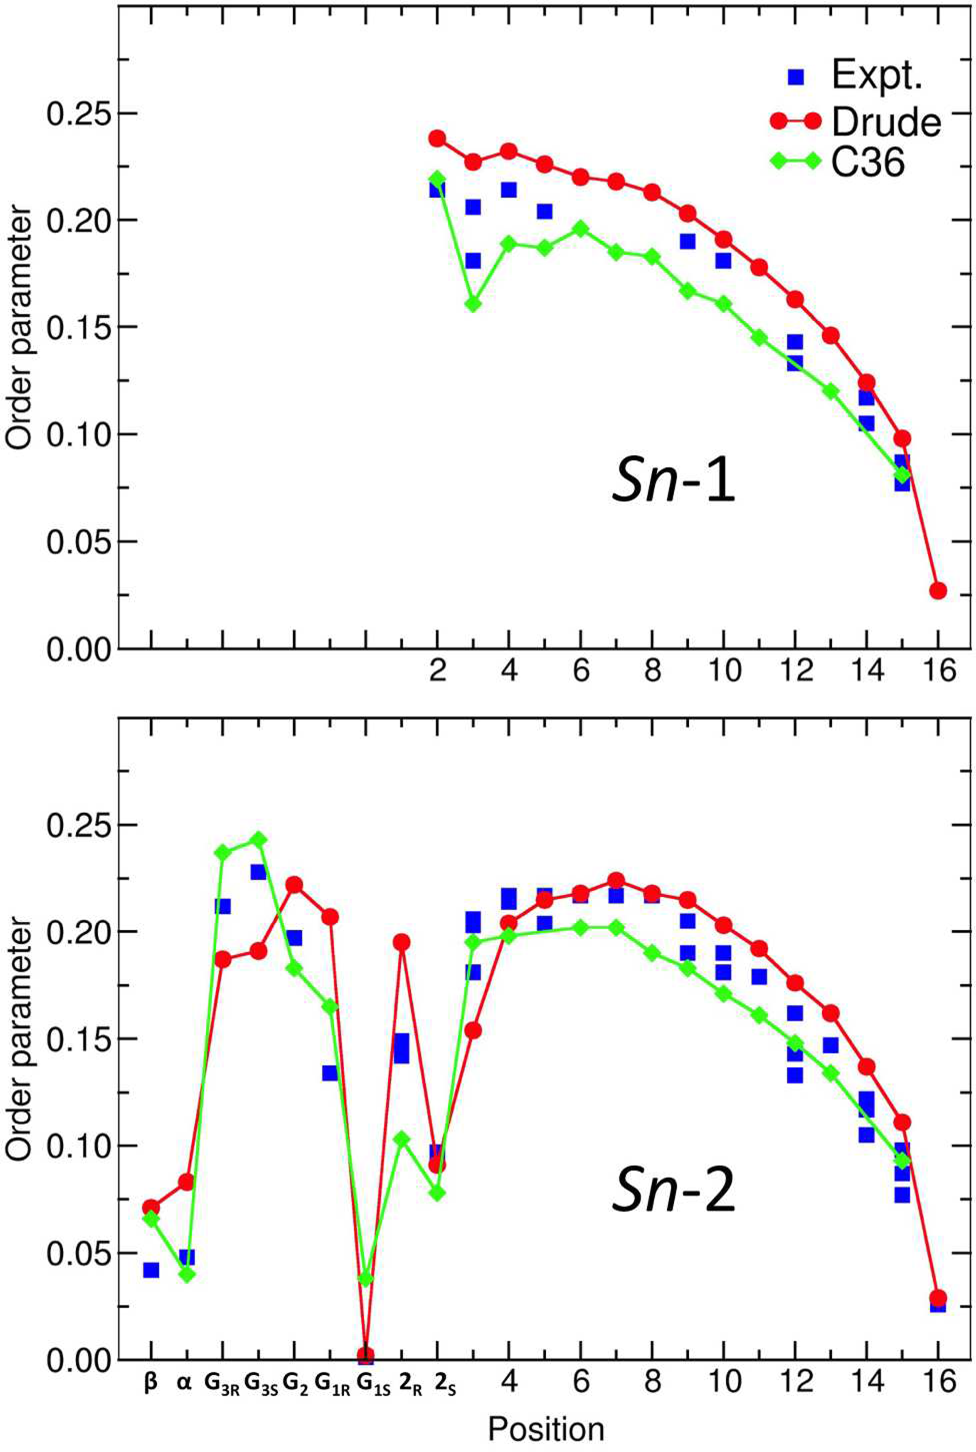
\includegraphics[width=\columnwidth]{../Figures/dppc_order_parameters_drude.png}
  \caption{NMR deuterium order parameter ($S_\mathrm{CD}$) values for a
  	hydrated DPPC bilayer from Ref.~\citenum{li2017drude}. Shown are the $S_\mathrm{CD}$ calculated using the new
  	Drude polarizable force field (red), C36 additive force field (blue), and
  	measured from experiments (black). The results for the C36 force field
  	were taken from Klauda \textit{et al.}~\cite{klauda2010update}. Experimental data were taken from Seelig and co-workers~\cite{seelig1974dynamic,seelig1975bilayers,gally1975conformation,gally1981structure} and Strenk \textit{et al.}~\cite{strenk1985model}; the data for the Sn-2 chain is taken from Douliez and \textit{et al.}~\cite{douliez1995restatement}}
  \label{fig:drudedppc}
\end{figure}

\begin{figure}[!htb]
	\centering
	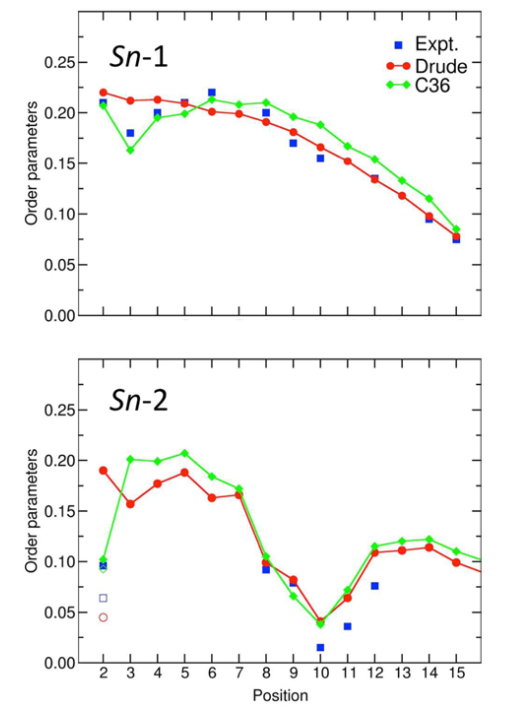
\includegraphics[width=\columnwidth]{../Figures/popc_order_parameters_drude.png}
	\caption{NMR deuterium order parameters ($S_\mathrm{CD}$) for a hydrated
		POPC bilayer from Drude polarizable force field~\cite{li2017drude}. Shown are the $S_\mathrm{CD}$ calculated using the new Drude
		polarizable force field (red), C36 additive force field (blue), and
		measured from experiments (black). The results for the C36 force field were taken from Klauda \textit{et.al.}~\cite{klauda2010update}. The MD values were calculated at 303 K. The experimental data collected at 300 K is from Seelig and Seelig~\cite{seelig1975bilayers}. The open symbols at position 2 of the Sn-2 chain represent the split values of the order parameters for HR and HS.}
	\label{fig:drudepopc}
	\end{figure}
		
\begin{figure}[!hbt]
	\centering
	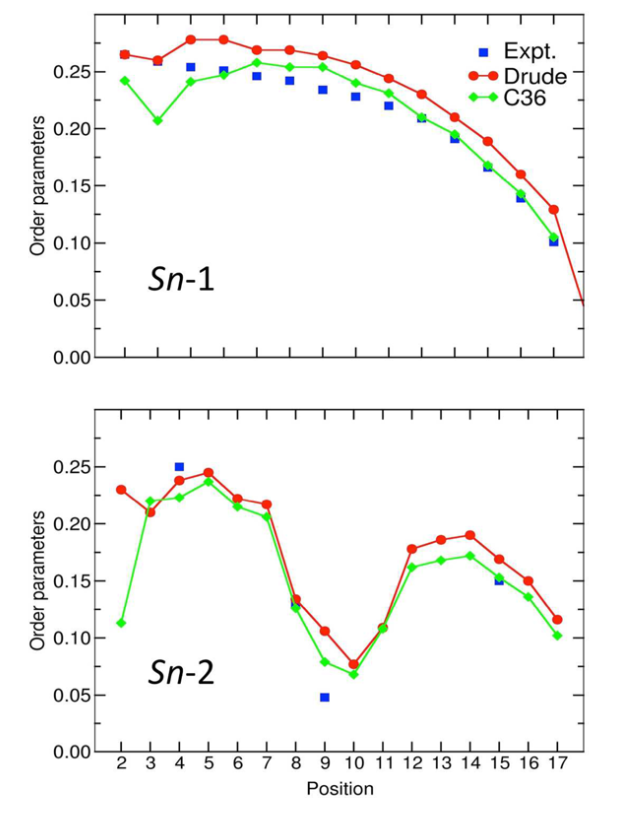
\includegraphics[width=\columnwidth]{../Figures/pope_order_parameters_drude.png}
	\caption{NMR deuterium order parameters ($S_\mathrm{CD}$) for a hydrated POPE bilayer. Shown are the $S_\mathrm{CD}$ calculated using the new Drude
		polarizable force field at 303 K (red), C36 additive force field at 310 K
		(blue), and measured from experiments at 310 K (black). The results for the C36 force field were taken from Klauda \textit{et al.}~\cite{klauda2010update}. The experimental data are taken from~\cite{shaikh2002monounsaturated,perly1985acyl}.}
	\label{fig:drudepope}
	\end{figure}
			
The Atomic Multipole Optimized Energetics for Biomolecular Applications (AMOEBA)
force field is based on representing the charge distribution of each atom by
atomic monopole, dipole, and quadrupole moments. The literature in this case a
bit scattered, but so far I managed to dig out force field parameters for DMPG~\cite{chu2018anionicpolarizable},
POPS~\cite{chu2018anionicpolarizable}, DOPC~\cite{chu2018polarizable}, and POPE~\cite{chu2018polarizable}. In the original paper the deuterium order
parameters have been reported without the signs and the reported experimental
values are sparse (Fig.~\ref{fig:amoebadopc}).

\begin{figure}[!hbt]
  \centering
  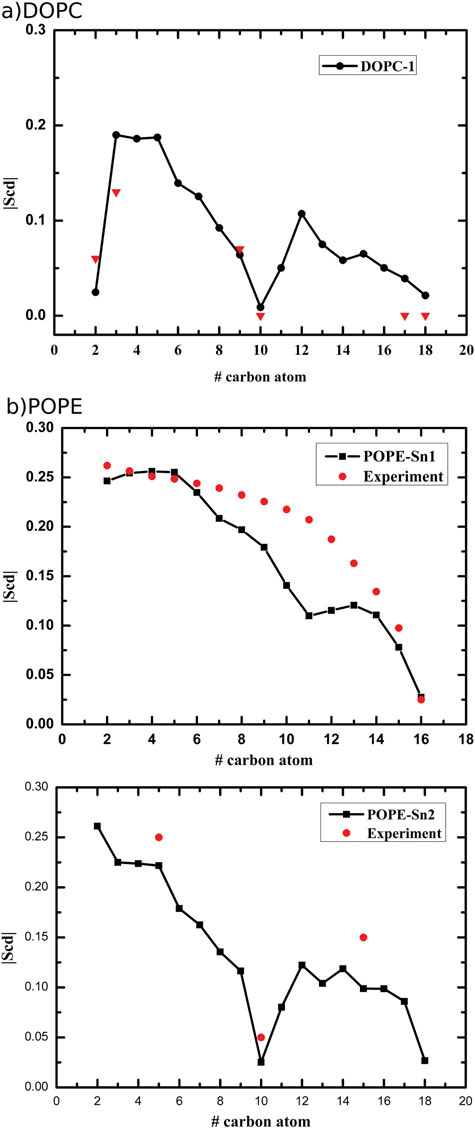
\includegraphics[width=\columnwidth]{../Figures/order_parameter_amoeba.png}
  \caption{NMR deuterium order parameters for DOPC and POPE lipids from AMOEBA
  force field~\cite{chu2018polarizable}.The order parameters for the DOPC and POPE bilayer system averaged over the last 20~ns simulations (a) Sn-1, (b) Sn-2, are compared with the experimental values that are shown in red~\cite{seelig1978molecular,perly1985acyl,shaikh2002monounsaturated}.}
\label{fig:amoebadopc}
\end{figure}

\begin{figure}[!hbt]
	\centering
	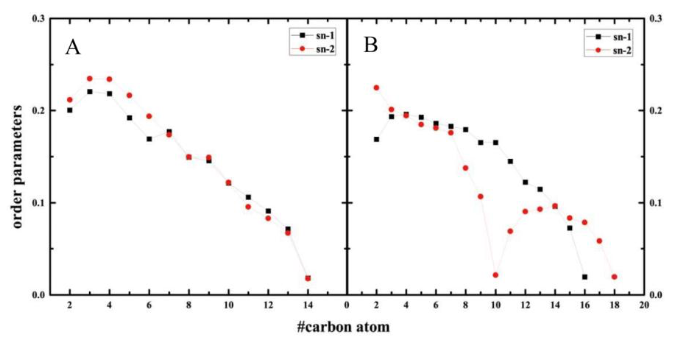
\includegraphics[width=1.05\columnwidth]{../Figures/dmpg_pops_order_parameters_amoeba.png}
	\caption{The order parameters for bilayer system averaged over the last 20 ns simulations from the AMOEBA force field~\cite{chu2018anionicpolarizable}. (A) The
		order parameters for DMPG bilayer system; (B) The order parameters for POPS bilayer system. order parameters for DMPG bilayer system; (B) The order parameters for POPS bilayer system.}
	\label{fig:amoebadmpg}
\end{figure}

CHARMM-Fluctuating Charge/Charge equilibration (FQ/CHEQ, the name has changed a
few times over the course of development) force field allows the magnitude of
the individual atomic partial charges to change over the course of a simulation
by assigning a fictitious mass to each of the charges and treating them as
additional degrees of freedom in the equations of motion. So far, I managed to
find the force field parameters for DMPC~\cite{davis2009molecular} and DPPC~\cite{davis2009charge}. However, further work
on this force field, especially for the lipids, seems have ceased. The order parameters reported in these papers are given in Figs.~\ref{fig:dmpccheq}-\ref{fig:dppccheq}.

\begin{figure}[!hbt]
  \centering
  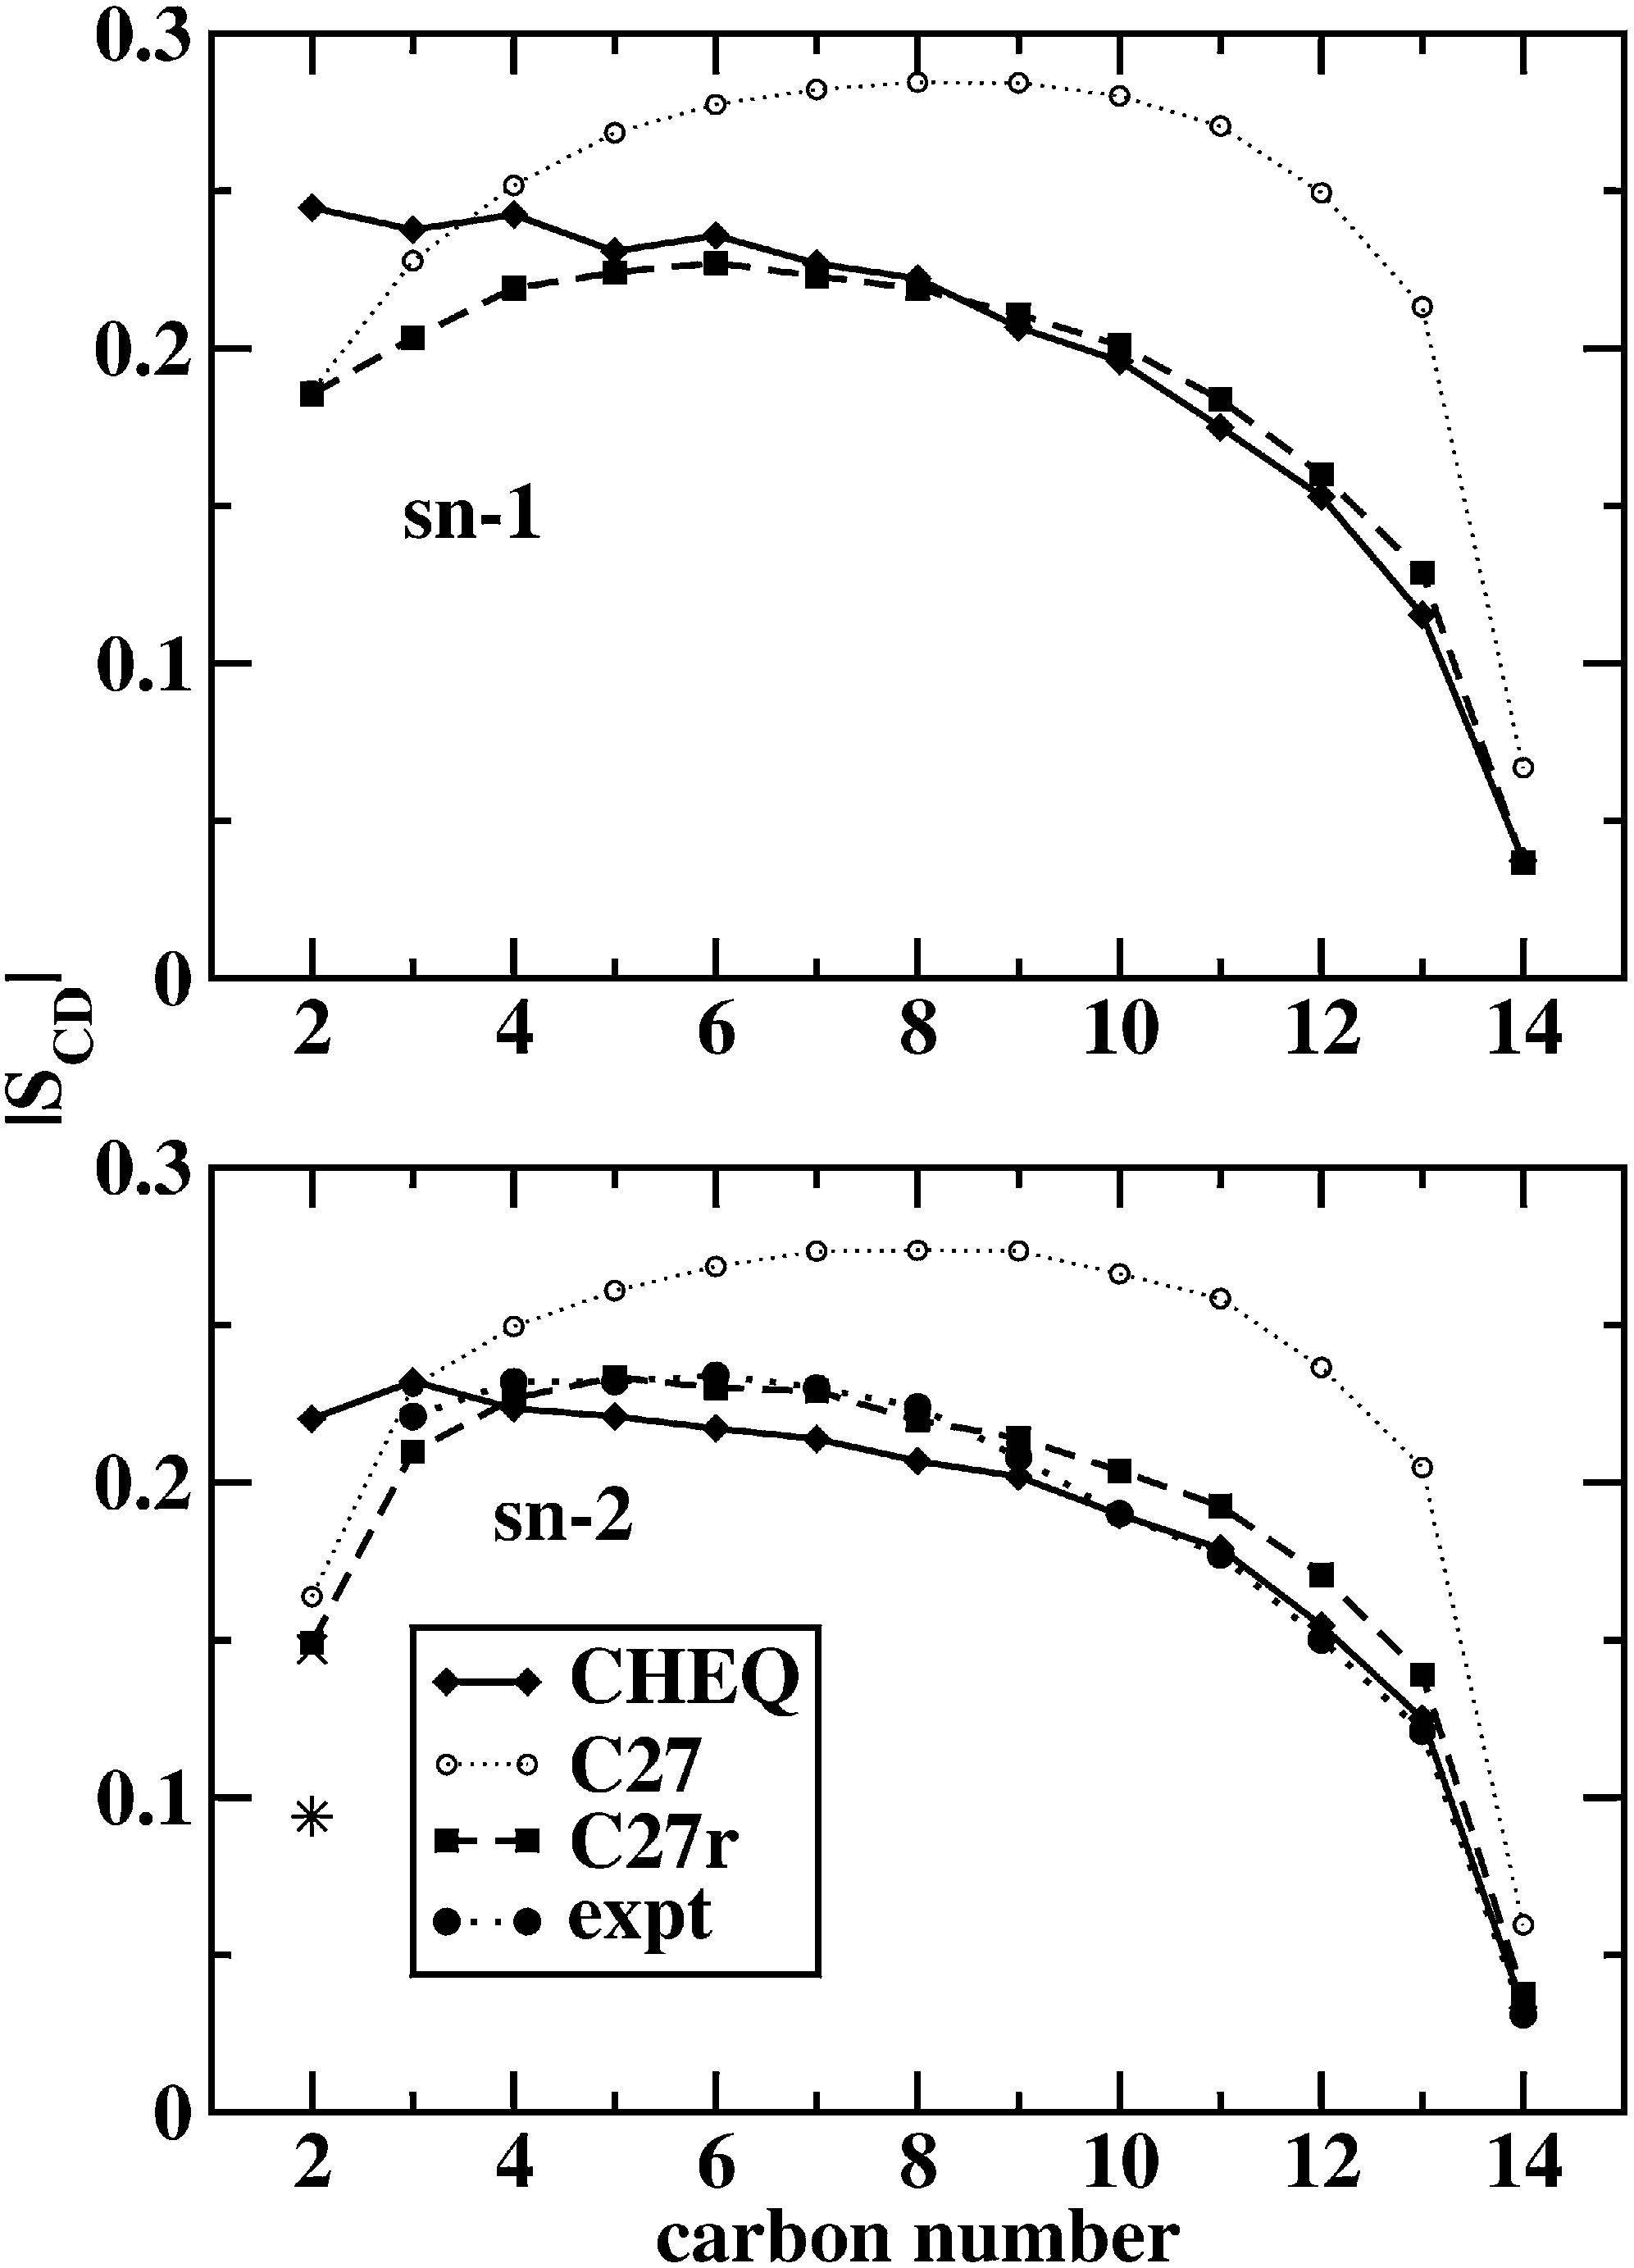
\includegraphics[width=\columnwidth]{../Figures/dmpc_order_charmmfq.png}
  \caption{Deuterium order parameters for the tail groups of DMPC as a function of position on the sn-1 (upper) and sn-2 (lower) hydrocarbon chain from CHEQ force field~\cite{davis2009molecular}. Values are shown for the polarizable (CHEQ) and nonpolarizable (C27) models, as well as for the revised CHARMM force field for alkanes (C27r)~\cite{klauda2005ab}. Experimental data~\cite{douliez1995restatement} for the asymmetric sn-2 chain (lower) are also shown, with the star and X symbols marking the values for the 2R and 2S hydrogens, respectively.}
  \label{fig:dmpccheq}
\end{figure}

\begin{figure}[!hbt]
	
	\centering
	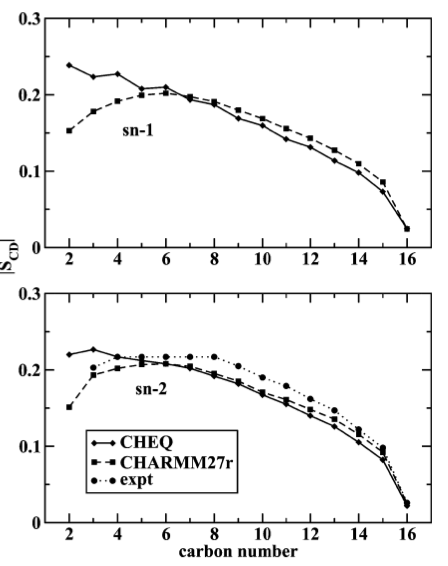
\includegraphics[width=\columnwidth]{../Figures/dppc_order_parameters_cheq.png}
	\caption{Magnitude of the deuterium order parameters for the tail groups as a function of position along the hydrocarbon chain for the DPPC from CHEQ force field~\cite{davis2009charge}. Values are shown for the polarizable CHEQ and nonpolarizable CHARMM27r models. Experimental data is also shown~\cite{douliez1995restatement}.}
	\label{fig:dppccheq}
	
\end{figure}

Currently, I continue reviewing the polarizable force field literature. This could reveal additional force fields to those mentioned above. Please feel free to contribute with your knowledge and comments.

\section{Workflow and Data Contributions}
%Among the force fields I mentioned, CHARMM-Drude seems to be the
%most commonly and actively used. AMOEBA and CHARMM-FQ force fields have
%limited number of lipids in their databases, and particularly for the CHARMM-FQ
%it looks like no significant further work is done. Based on these, I would suggest us to focus mostly on the CHARMM-Drude and to use the data from the other force fields whene%ver they have the
%parameters.\\

Due to the limited number of force fields and available lipids, I suggest
doing something similar to the NMRLipids II and IV projects combined: Checking
the performance of all force fields for available zwitterionic and charged head
groups employing the NMR C--H bond order parameters, X-ray form factors, and ion binding. %, and correlation times.

%For the last year, as the NMRLipids community we have developed a Python script that performs the required calculations for the order parameters, X-ray form factors, and correlation times. Our current idea is to utilize this script and make it the main analysis source for this project. We are making the final touches to the script and we will make it available soon.\\

%Concerning the data contributions. We will be creating a public GitHub repository within the NMRLipids for this project. The Python script and its documentation/user guide will be available in this repository. We kindly ask everyone who are willing to contribute with their trajectories to upload them to the NMRLipids community on Zenodo. From there, you can analyse your trajectories using our Python script. Final step would be to upload the results, but not the trajectories, to the project's GitHub repository. Please comment under this post if you are willing to run/upload simulations.\\

The overall workflow of this project will be based on the NMRlipids principles. All contributors, regardless of their level of contribution, will be offered a coauthorship when we start writing the manuscript. I will be a corresponding author, i.e. assume the role Samuli had in previous NMRLipids projects.

%\section{Methods}
\subsection{Data contributions}

In order to automatize the analysis and reduce the human effort, we have compiled a Python script, {\tt AddData.ipynb}, available at the {\tt scripts} folder of the \href{https://github.com/NMRLipids/NMRlipidsVIpolarizableFFs}{NMRlipids IV GitHub repository}. The script reads trajectories from any public repository using the unique Digital Object Identifier (DOI), does the necessary preprocessing, calls other scripts ({\tt Order\-Parameter.py}) %, {\tt corr\_ftios\_ind.sh}, and {\tt corrtimes.py})
to calculate the C--H bond order parameters, %and effective correlation times,
and writes the output to a directory with a unique name derived from the data set DOI.

{\tt AddData.ipynb} requires the simulation description to be supplied by the user. This part is located in the beginning of the script, where the user needs to define
1) the data set DOI,
2) the file that contains the atom indexing for calculating the order parameters,
3) the employed software,
4) the employed force field,
5) the force field source,
6) the names of the trajectory files, and finally
7) the working directory where the output will be written.
Output of {\tt AddData.ipynb} then is a uniquely (based on the DOI) named directory that contains a {\tt README} file plus files that contain the order parameters. No changes/alterations to the files or the file names will be necessary.

Currently, {\tt AddData.ipynb} is capable of processing and analyzing the trajectories in {\tt xtc} (Gromacs) and {\tt dcd} (NAMD) formats. In case your trajectories are in a different file format, please either make the necessary changes to the {\tt AddData.ipynb} and push it back to the GitHub repository, or \href{mailto:b.kav@fz-juelich.de}{email me} so that we can handle your request and update the script according to your data format.

For {\tt AddData.ipynb} to work, it needs two additional Python libraries, \href{http://mdtraj.org/1.9.3/}{MDTraj} and \href{http://mdanalysis.org}{MDAnalysis}, to be installed on your computer. MDAnalysis is required by the {\tt OrderParameter.py}. MDTraj is required to convert trajectories, in case they differ from the {\tt xtc} format.%, to {\tt xtc} format so that the {\tt AddData.ipynb} can function.

\subsection{Authorship and Data Ownership}
Any contribution---a comment on the blog, adding a few lines to the analysis scripts, or supplying raw data---is invaluable!
The NMRlipids \href{https://nmrlipids.blogspot.com/p/blog-page_2.html}{rules on authorship} will be followed, that is, all contributors to the project will be offered coauthorship on the final publication.

As a data contributor, you maintain rights on your data set according to the licensing option you choose on the public server where you upload your data. We encourage using the Creative Commons licensing scheme (whichever version suits you) and making your data set publicly available to whomever needs it. In particular, by submitting your data set to the NMRlipids community on Zenodo, you agree your data to be used in the NMRlipids projects. Important: Please make sure that the data server you use for uploading your data set generates a DOI.



%\section{References}
\bibliography{references.bib}


\end{document}
